\chapter[Kaggle]{Kaggle}
\section{Introducción.}
\subsection{Descripción del problema.}
Los atributos son los siguientes
\begin{itemize}
	\item ip
	\item app
	\item device
	\item so
	\item click\_time
	\item attributed\_time
	\item is\_attributed
\end{itemize}
\subsection{Limitaciones encontradas.}
La principal limitación hardware que he encontrado es el uso de memoria RAM debido al gran tamaño del conjunto de entrenamiento (7.7 GB).
\subsection{Herramientas utilizadas}
Boosting es un enfoque donde el resultado se da usando la media
ponderada de varios árboles y combina las ventajas de cada árbol al darle
a éste un peso en la decisión final. En este enfoque, los árboles tienen
que ir construyéndose de manera lineal para intentar añadir árboles que
mejoren aquello en lo que el resto ha fallado. El objetivo final es eliminar el
sesgo. [9]
Para la competición en particular, se ha usado la librería XGBoost,
que nos permite usar Boosting con árboles de forma paralela, eficiente y
flexible. Este ha sido el algoritmo usado en el resultado final debido a su
capacidad para obtener valores significativamente superiores a Random
Forest, aunque sacrificando velocidad en el entrenamiento.
He usado los siguientes bibliotecas
\begin{itemize}
	\item xgboost
	\item matplotlib
	\item pandas
	\item numpy
\end{itemize}
\section{Objetivos.}
\section{Estudio de los datos.}
Para poder elegir una estrategia para el preprocesamiento es necesario realizar una visualización de los datos. De esta forma, podremos obtener cómo están distribuidos los valores de cada uno de los atributos o si existe alguna relación de correlación entre ellos. Para poder realizar este estudio correctamente separaremos los atributos de tipo fecha en dia,mes y año.
\begin{figure}[H]
	\centering
	\begin{subfigure}{.5\textwidth}
		\centering
		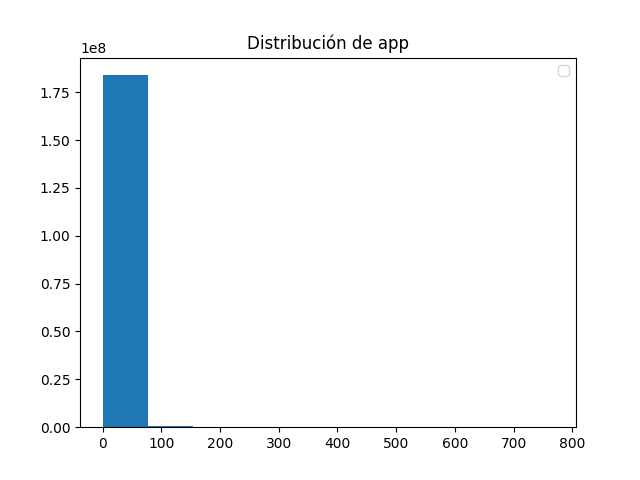
\includegraphics[scale=0.5]{img/app_distribution.png}
		\caption{A subfigure}
		\label{fig:sub1}
	\end{subfigure}%
	\begin{subfigure}{.5\textwidth}
		\centering
		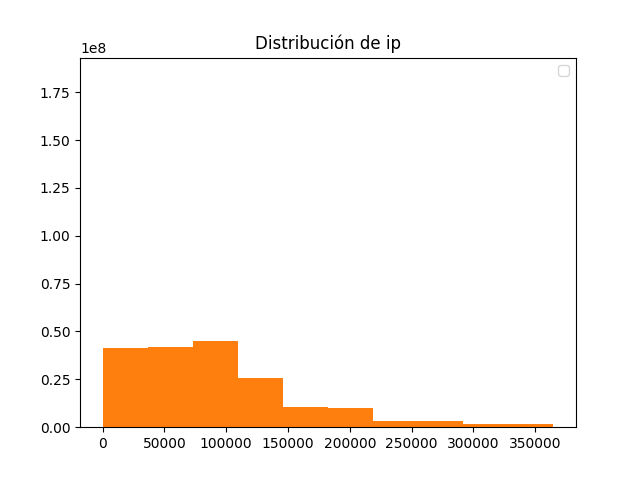
\includegraphics[scale=0.5]{img/ip_distribution.png}
		\caption{A subfigure}
		\label{fig:sub2}
	\end{subfigure}
	\caption{A figure with two subfigures}
	\label{fig:test}
\end{figure}
\begin{figure}[H]
	\centering
	\begin{subfigure}{.5\textwidth}
		\centering
	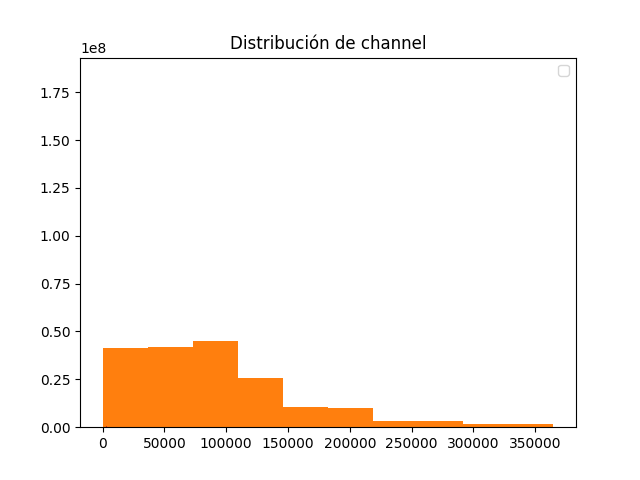
\includegraphics[scale=0.5]{img/channel_distribution.png}
		\caption{A subfigure}
		\label{fig:sub1}
	\end{subfigure}%
	\begin{subfigure}{.5\textwidth}
		\centering
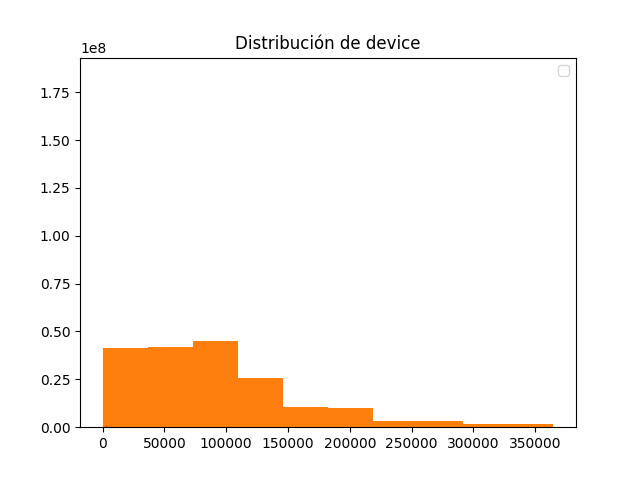
\includegraphics[scale=0.5]{img/device_distribution.png}
		\caption{A subfigure}
		\label{fig:sub2}
	\end{subfigure}
	\caption{A figure with two subfigures}
	\label{fig:test}
\end{figure}

\begin{figure}[H]
	\centering
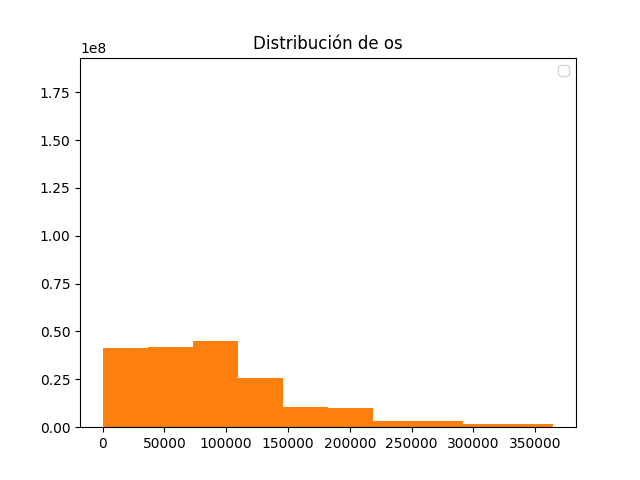
\includegraphics[scale=0.5]{img/os_distribution.png}
\caption{A figure with two subfigures}
\label{fig:test}	
\end{figure}
En las gráficas anteriores podemos observar que las variables app,channel,device,ip y os se d
\medskip
Ahora, estudiaremos la variable click\_time. Al tratarse de una variable que representa una hora y fecha, la dividiremos en día,mes,año y valor timestamp(segundos transcurridos desde una fecha fijada por el sistema operativo).
\begin{figure}[H]
	\centering
	\begin{subfigure}{.5\textwidth}
		\centering
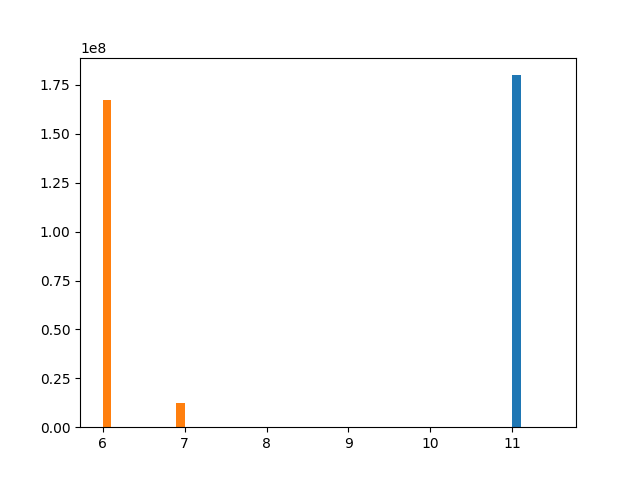
\includegraphics[scale=0.45]{img/click_time_day_distribution.png}
		\caption{A subfigure}
		\label{fig:sub1}
	\end{subfigure}%
	\begin{subfigure}{.5\textwidth}
		\centering
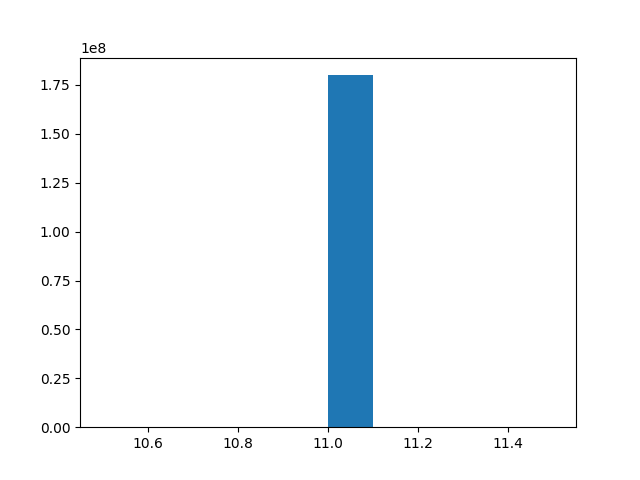
\includegraphics[scale=0.45]{img/click_time_month_distribution.png}
		\caption{A subfigure}
		\label{fig:sub2}
	\end{subfigure}
	\caption{A figure with two subfigures}
	\label{fig:test}
\end{figure}
\begin{figure}[H]
	\centering
	\begin{subfigure}{.5\textwidth}
		\centering
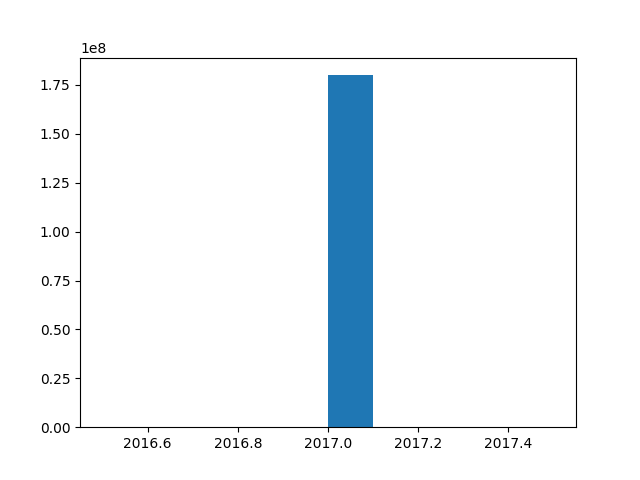
\includegraphics[scale=0.5]{img/click_time_year_distribution.png}
		\caption{A subfigure}
		\label{fig:sub1}
	\end{subfigure}%
	\begin{subfigure}{.5\textwidth}
		\centering
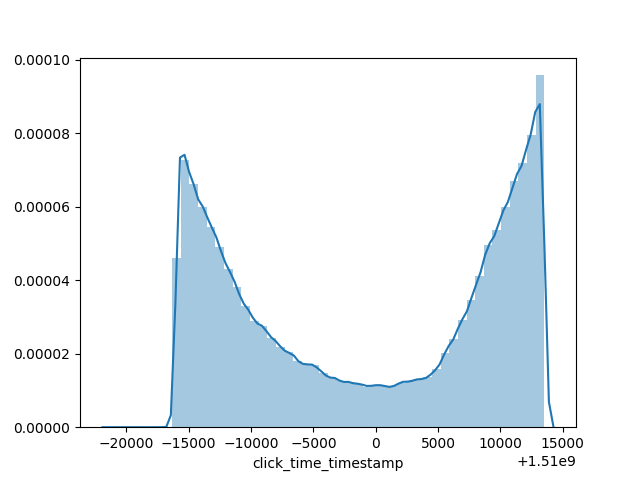
\includegraphics[scale=0.5]{img/normalDistclick_time_timestamp.png}
		\caption{A subfigure}
		\label{fig:sub2}
	\end{subfigure}
	\caption{A figure with two subfigures}
	\label{fig:test}
\end{figure}

En esta ocasión si podemos establecer valores fijos para algunos campos:
\begin{enumerate}
	\item Los días son el 6,7 y 11
	\item Todos los valores corresponden al mes 11.
	\item Todos los registros corresponden al año 2017
\end{enumerate}

Finalmente, estudiaremos el balanceo de clases de la variable a clasificar. Cabe recordar que un desbalanceo de clases provocará que el modelo de aprendizaje que construiremos no clasifica bien para las clases minoritarias.
\begin{figure}[H]
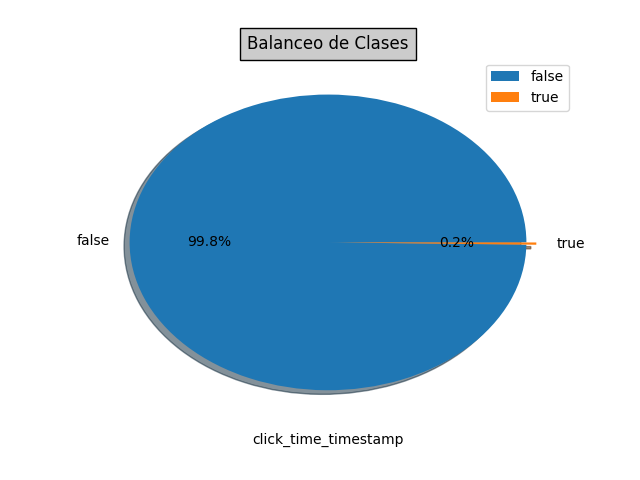
\includegraphics[scale=0.75]{img/imbalacing.png}
\label{}
\caption{Balanceo de clases}
\end{figure}
Por otro lado, estudiaremos el número de valores desconocidos de cada columna ya que un atributo con un gran número de valores desconocidos no nos proporciona información valiosa. Los resultados obtenidos son los siguientes.
\begin{table}[H]
	\centering
	\begin{tabular}{lllll}
	Atributo& Total & \%    \\
	ip	& 0 &0 \\
	app	& 0 & 0   \\
	os	& 0 & 0 \\
	chanel &0 & 0 \\
	device & 0 & 0  \\
	click\_time& 0& 0 \\
	attributed\_time &184447044& 0.997529
	\end{tabular}
	\caption{}
\label{}
\end{table}
\section{Preprocesamiento.}
En este tipo de competiciones la fase de preprocesamiento suele ser la que marca más la diferencia. Esto es debido a que a igualdad de capacidad de procesamiento, se puede obtener la configuración de parámetros óptima para los algoritmos usados, siendo los algoritmos usados similares entre los participantes.
\medskip
Para evaluar la bondad de las decisiones tomadas haremos uso de la clasificación mediante boosting, debido a que nos permite ver la importancia de cada atributo a la hora de construir el modelo de aprendizaje. Esto nos permitirá discriminar que cambios nos proporcionan mejoras.
\medskip
Los resultados obtenidos en la sección anterior nos llevan a tomar las siguientes decisiones:
\begin{itemize}
	\item Eliminar la columna attributed\_time
	\item Eliminar las columnas mes y año provenientes de click\_time
\end{itemize}
A continuación, vamos a  seguir trabajando con la variable click\_time los siguientes cambios a probar son introducir el día de la semana y la hora.
Finalmente, realizaremos algunas agrupaciones añadiendo una columna que contabilize el número de instancias coincidentes:
\begin{itemize}
	\item ip-day-hour
	\item ip-app
	\item ip-app-os	
\end{itemize}
Los resultados obtenidos en las distintas fases de preprocesamiento se muestran en la siguiente tabla.
\begin{table}[]
	\centering
	\caption{My caption}
	\label{my-label}
	\begin{tabular}{lllll}
		Cambio realizado& Resultado & Importancia del cambio introducido &  &  \\
		&  &  &  &  \\
		&  &  &  &  \\
		&  &  &  & 
	\end{tabular}
\end{table}
\section{Soluciones planteadas.}
\subsection{}
Para la búsqueda de los mejores parámetros en cada clasificador, se
aplica el concepto de Grid Search. Esto significa que podemos hacer bucles
para explorar con diferentes valores y combinaciones de parámetros. Si
tenemos suficiente capacidad de procesamiento, es lo ideal a la hora de
optimizar los parámetros, pero, como es de esperar, es una operación muy
pesada.
\subsection{RUSBoosting}
\begin{algorithm}
\end{algorithm}
\subsection{CUSBoosting}
\begin{algorithm}
\end{algorithm}
\subsection{MIX}
\subsection{Resultados obtenidos.}
\section{Conclusiones obtenidas.}
\subsection{Cosas que se quedaron por hacer.}
